%A good requirement is:
%*Correct
%*Unambiguous (all statements have exactly one interpretation)
%*Complete (where TBDs are absolutely necessary, document why the information is unknown, who is responsible for resolution, and the deadline)
%*Consistent
%*Ranked for importance and/or stability
%*Verifiable (avoid soft descriptions like “works well”, “is #user frndly”; use concrete terms and specify measurable #quantities)
%*Modifiable (evolve the Requirements Specification only via a #formal change process, preserving a complete audit trail of #changes)
%*Does not specify any particular design
%*Traceable (cross-reference with source documents and spawned documents).




\chapter{Requirement specification}

\section{Version history}
\begin{table}[H]
\begin{tabular}{|c|p{9cm}|c|c|}
\hline
Version & Description & Author & Date\\
\hline
0.1 & Initial draft & JK & 21/12-13\\
\hline
\end{tabular}
\end{table}

\section{Purpose and scope}
Formål og omfang samt anvendelse.

\section{References}
Referencer

\section{Glossary}
Ordforklaringer

\section{General description}

\subsection{General System}
\begin{figure}[H]
	\centering
	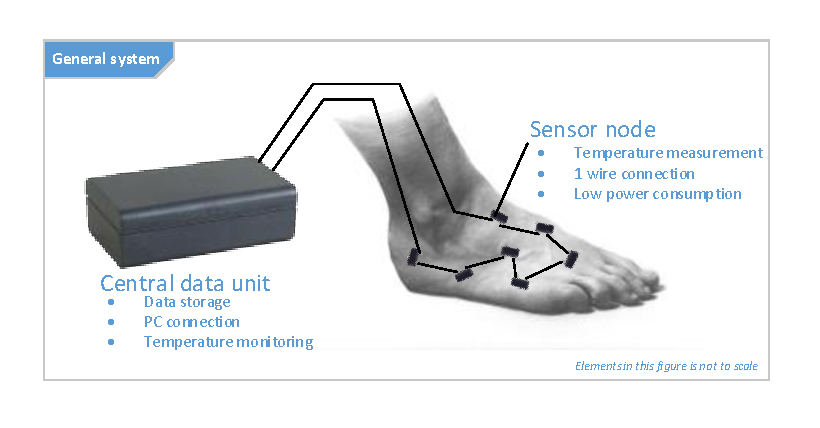
\includegraphics[width=0.8\textwidth]{billeder/GeneralSystem}
	\caption{General System}
\end{figure}

\subsection{System description}
Et device der skal påmonteres foden på en person der er disponeret til at udvikle Charcotfod. Devicet skal ud fra temperatur og aktivitetsniveau finde ud af om der er en fare for overbelastning. Hvis dette er tilfældet skal brugeren advares.

\subsection{Constraints}

\subsection{Dependencies}

%\subsection{Prototype af UI eller GUI}

%\subsection{Beskrivelse af UI eller GUI}

\section{Functional requirements}
Below is listed all functional requirements to the system.\\
\textbf{\large{Priority definitions}}\\
The following definitions are intended as a guideline to prioritize requirements.
\begin{itemize}[noitemsep,nolistsep]
\item Priority 1 - This is a "Need to Have" either defined by law or of most importance of the project.
\item Priority 2 - This requirement is if high importance and will be of great benefit for the system
\item Priority 3 - This requirement will be great to have but not important
\item Priority 4 - This requirement is purely "Nice-to-have" and will not be considered unless there is time to spare.
\end{itemize}

\subsection{Actor diagram}
Visio actor diagramme.

\subsection{Actors of the system}
\begin{table}[H]
	\centering
	\begin{tabular}{|l|p{7cm}|}
	\hline
	Actor name & Central data unit \\ \hline
	Type & Primary \\ \hline
	Description & asdf dsdf \\ \hline
	\end{tabular}
\end{table}

\begin{table}[H]
	\centering
	\begin{tabular}{|l|p{7cm}|}
	\hline
	Actor name & Sensors \\ \hline
	Type & Primary \\ \hline
	Description & asdf dsdf \\ \hline
	\end{tabular}
\end{table}

\subsection{Use Case diagram}
Visio again.

\subsection{Use Case diagram}
\subsubsection{Read data from sensor \#X}
\begin{table}[H]
	\centering
	\begin{tabular}{|l|p{7cm}|}
	\hline
	Goal & asdf dsdf \\ \hline
	Initialisation & asdf dsdf \\ \hline
	Actors & asdf dsdf \\ \hline
	Reference & asdf dsdf \\ \hline
	\# of concurrent events & asdf dsdf \\ \hline
	Prerequisite  & asdf dsdf \\ \hline
	Post condition & asdf dsdf \\ \hline
	\multirow{3}{*}{Main Scenario} & 1. Henning \\
	& 2. Henning\\
	& 3. Henning\\ \hline
	\multirow{1}{*}{Exceptions} & 1. Henning \\ \hline
	\end{tabular}
\end{table}


\subsection{System Features}
Below is listed all functional requirements.

\subsubsection{Use cases}
\section{Non functional requirements}

\subsection{General requrements}

\subsection{Temperature sensor requirements}

\subsubsection{Functionality Requirements}

\subsubsection{Hardware Requirements}
Krav til hardware (if any)\\
*Power consumption\\
*Performance\\
*Maintainability\\
*Interfaces\\
*Accuracy\\
\subsubsection{Software Requirements}
Krav til software (if any)\\
*Performance\\
*Maintainability\\
*Interfaces\\
*Language??\\

\subsubsection{External interfaces}
N/A
\subsection{Main data collection unit requirements}

\subsubsection{Functionality Requirements}

\subsubsection{Hardware Requirements}
Krav til hardware (if any)\\
*Power consumption\\
*Performance\\
*Maintainability\\
*Interfaces\\
*Accuracy\\

\subsubsection{Software Requirements}
Krav til software (if any)\\
*Performance\\
*Maintainability\\
*Interfaces\\
*Language??\\

\subsubsection{External interfaces}
*USB?\\
*UART?\\
*EEPROM?\\
*Flash?\\

\subsection{Project requirements}

\subsubsection{Documentation}
\begin{itemize}
\item Engelsk
\item SysML
\end{itemize}

\subsubsection{Technologies and tools}
\begin{itemize}
\item Matlab
\item Maple/Mathcad
\item Microsoft Visio 2010/2013
\item TortoiseSVN
\item TeXmaker
\end{itemize}

\subsubsection{Misc}
\begin{itemize}
\item Report is written in LaTeX.
\end{itemize}

\section{Non functional requirements}
(?) betyder at jeg ikke lige ved hvordan det skal specificeres eller om det overhovedet er et reelt krav.\\
\subsection{system requirements }
%%%%%%%%%%%%%%%%%%%%
% Generelle krav %
%%%%%%%%%%%%%%%%%%%%
General Requirements:\\
\begin{itemize}
\item Systemet skal have en levetid på 1-3 år(specificitet)
\item Der skal tænkes på fremstillingspris(?)
\end{itemize}
%%%%%%%%%%%%%%%%%%%%
% Sensor krav %
%%%%%%%%%%%%%%%%%%%%
Sensor requirements:\\
\begin{itemize}
\item Målesensoren skal have en nøjagtighed på $\pm0.5 ^{\circ}C$
\item Accelerometer
\item Kalibrering(?)
\end{itemize}
%%%%%%%%%%%%%%%%%%%%
% Central dataopsamling%
%%%%%%%%%%%%%%%%%%%%
Central data collection unit:\\
\begin{itemize}
\item Clock speed
\item GPIO amount
\end{itemize}

%Teksturdesign:\\
%\begin{itemize}
%\item Sokken skal være meget elastisk(?)
%\item Sokken skal kunne anvendes hele dagen(?)
%\item Sokken skal kunne avnendes med fodtøj(?)
%\item Sokken skal kunne rengøres (?)
%\end{itemize}

\subsection{Communication requirements}
\begin{itemize}
\item 0 - 12 VDC $\pm$0.5VDC
\item 500 mA $\pm$25mA
\end{itemize}

\subsection{Interfaces Requirements}
prototyper af PC og/eller smartphone\\
Datastik så data kan tages ud af enheden for debugging purpose.\\

\subsection{Development and technology requirements }
V-model:\\
\begin{itemize}
\item Modificeret Scrum til styringsprocessen for sprint mellem hver projektmilestone
\item Henvisning til tidsplan og milestones
\end{itemize}

Documentation:\\
\begin{itemize}
\item Engelsk
\item SysML
\end{itemize}

Technologies and tools:\\
\begin{itemize}
\item Matlab
\item Maple/Mathcad
\item Microsoft Visio 2010/2013
\item TortoiseSVN
\item TeXmaker
\end{itemize}

Misc:\\
\begin{itemize}
\item Report is written in LaTeX.
\end{itemize}
\section{List of figures}